\chapter{\label{lesson6}Передаточное соотношение}
{\bfseries Анонс:}\\\\
Передаточное соотношение. Соотношение на скорость. Соотношение на мощность. Запускающий механизм для волчка.\\\\
{\bfseries Цели:}
\begin{itemize}
	\item{}{\bfseries Обучающие:} Закрепить понятия угловая и линейная скорости, частота, период. Познакомить учащихся с понятием передаточного соотношения и видами передач.
	\item{}{\bfseries Развивающие:} Формирование умений сравнивать, классифицировать, обобщать изучаемые факты и понятия. Развитие познавательного интереса для учащихся.\\
\end{itemize}	
{\bfseries Ход занятия:}\\\\
\begin{tabular}{lll}
	\hyperlink{lesson6x1}{1. Организационный момент} & Презентация & (5 мин)\\
	\hyperlink{lesson6x2}{2. Движение по окружности} & Практика & (5 мин) \\
	\hyperlink{lesson6x3}{3. Передаточное соотношение} & Презентация & (50 мин) \\
	\hyperlink{lesson6x4}{4. Решение задач} & Практика & (30 мин)\\
	\hyperlink{lesson6x5}{5. Запускающий механизм волчка} & Игра & (30 мин)
\end{tabular}\\\\

{\hypertarget{lesson6x1}{\blackBlueText{I.Организационный момент}}}\\\\

Для первой части сегодняшнего занятия понадобятся тетради с предыдущей теорией. Для практикума по запуску волчка у каждого должен быть отдельный набор и рабочий стол для сбора и тестирования конструкции.\\\\

{\hypertarget{lesson6x2}{\blackBlueText{II. Движение по окружности}}}\\\\	

В качестве легкой разминки предлагается ряд устных вопросов по предыдущему материалу:

\begin{enumerate}
	\item Минутная стрелка часов делает один полный оборот. Чему равен период обращения?
	\begin{enumerate}
		\item 60 c;
		\item 1/3600 с;
		\item 3600 с.
	\end{enumerate}
	\item Колесо велосипеда делает один оборот за 4 с. Определите частоту вращения.
	\begin{enumerate}
		\item 0,25 1/с;
		\item 4 1/с;
		\item 2 1/с.
	\end{enumerate}
	\item  Винт моторной лодки делает 25 оборотов за 1 с. Чем, равна угловая скорость винта?
	\begin{enumerate}
		\item 25 рад/с;
		\item  \(\pi\)/25 рад/с;
		\item 50\(\pi\)рад/с.
	\end{enumerate}
	\item Определите частоту вращения сверла электрической дрели, если его угловая скорость равна 400 \(\pi\).
	\begin{enumerate}
		\item 800 1/с;
		\item 400 \(\pi\)1/с;
		\item 200 1/с.
	\end{enumerate} 
\end{enumerate}

{\bfseries Ответы  на тест:} в; а; в; в.
\clearpage
{\hypertarget{lesson6x3}{\blackBlueText{III. Передаточное соотношение}}}\\\\

В любой передаче линейные скорости крайних точек шестеренок совпадают. Тогда угловые скорости связаны соотношением:
\begin{figure}[h!]
	\begin{center}
		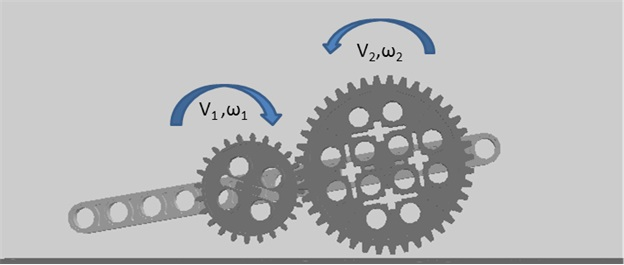
\includegraphics[width=1\linewidth]{chapters/chapter6/images/1}
		\caption{}
		\label{ris:image6x1}
	\end{center}
\end{figure}	
\begin{equation}
V_1=V_2\Rightarrow\omega_1 r_1=\omega_2 r_2\Rightarrow\frac{\omega_1}{\omega_2}=\frac{r_2}{r_1}=\frac{n_2}{n_1}=\iota_{12}    
\end{equation}

Для зубчатых и цепных передач радиусы относятся как число зубцов \(n_2\) и \(n_1\) (под первой шестеренкой здесь и далее понимается ведущая, под второй – ведомая). Это отношение обычно обозначают как \(\iota_12\)  и называют {\bfseries передаточным соотношением}.
\begin{equation}
\mbox{\underline{Для любознательных:} Доказать, что }\frac{r_2}{r_1}=\frac{n_2}{n_1}  
\end{equation}

Видно, что если \(\iota_{12}>1\), то скорость вращения в результате передачи понижается, и передача называется {\bfseries понижающей}.

Если  \(\iota_{12}<1\), то скорость вращения в результате передачи повышается, и передача называется {\bfseries повышающей}.

Но если мы выиграли в скорости, то в чем-то должны были проиграть? Все верно, {\bfseries во сколько раз выигрываем в скорости, во столько раз проигрываем в силе.}\\\\
\greenText{Инфографика}\\\\

В случае сложных систем, в передаче может быть задействовано несколько шестеренок. Возможны следующие варианты их расположения: шестеренки укреплены на одном валу.
\clearpage
\begin{figure}[h!]
	\begin{center}
		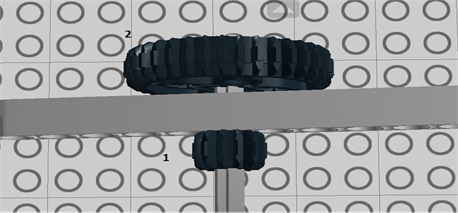
\includegraphics[width=1\linewidth]{chapters/chapter6/images/2}
		\caption{}
		\label{ris:image6x2}
	\end{center}
\end{figure}	

Или несколько шестеренок подряд сцеплено друг с другом.
\begin{figure}[h!]
	\begin{center}
		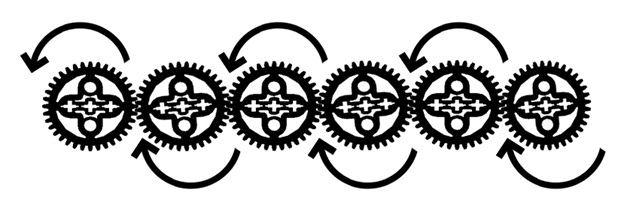
\includegraphics[width=1\linewidth]{chapters/chapter6/images/3}
		\caption{}
		\label{ris:image6x3}
	\end{center}
\end{figure}	

В первом случае (рис.~\ref{ris:image6x2}) совпадают угловые скорости вращения шестеренок, а линейные скорости краев относятся как их радиусы (число зубьев):
\begin{equation}
\omega_1=\omega_2\Rightarrow\frac{V_1}{r_1}=\frac{V_2}{r_2}\Rightarrow\frac{V_1}{V_2}=\frac{r_1}{r_2}=\frac{n_2}{n_1}
\end{equation}
\begin{equation}
\iota_{12}=1
\end{equation}

Передаточное соотношение в данном случае равно единице.

Можно показать, что при расчете сложной системы из многих шестеренок, можно пользоваться следующим правилом:

{\bfseries Передаточное соотношение системы равно произведению передаточных соотношений элементов системы.}
\clearpage
\begin{figure}[h!]
	\begin{center}
		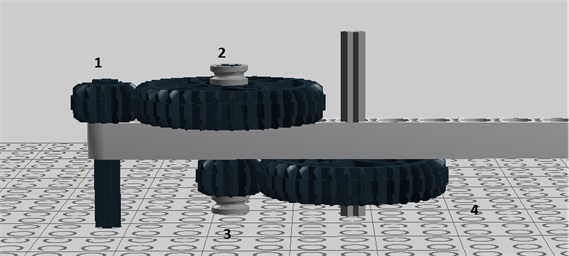
\includegraphics[width=1\linewidth]{chapters/chapter6/images/4}
		\caption{}
		\label{ris:image6x4}
	\end{center}
\end{figure}

\begin{equation}
\iota_{14}=\iota_{12}*\iota_{23}*\iota_{34}
\end{equation}

Отметим, что в данном примере \(\iota{23}=1\).

\underline{Для любознательных:} Доказать, правило (1). 

Применив это правило к системе, изображенной на \greenText{рис.~\ref{ris:image6x3}} получим:
\begin{equation}
\iota_{14}=\iota_{12}*\iota_{23}*\iota_{34}=\frac{n_1}{n_2}*\frac{n_2}{n_3}*\frac{n_3}{n_4}=\frac{n_1}{n_4}
\end{equation}

Получается «промежуточные» шестеренки здесь не играют никакой роли и могут быть любыми? Да, поэтому они носят название {\bfseries паразитные} шестеренки. Но, значит ли это, что такие шестеренки бессмысленны и подобные конструкции никогда не применяются? Нет, паразитные шестерни могут быть полезны как минимум в двух случаях:
\begin{itemize}
	\renewcommand{\textbullet}{\textendash}
	\item Передача вращения без изменения направления вращения. 
	\item Передача вращения на большое расстояние.\\\\
\end{itemize}

{\hypertarget{lesson6x4}{\blackBlueText{IV. Решение задач}}}\\\\

Теоретический материал из предыдущих пунктов рекомендуется дополнить решением задач. Часть из них может быть разобрана в классе, часть дана для самостоятельного изучения.
\begin{itemize}
	\renewcommand{\labelitemi}{\stepcounter{tasks}\Roman{tasks}.}
	\item Движение от шкива I (рис.~\ref{ris:image6x5}) к шкиву IV передается при помощи двух ременных передач. Найти частоту обращения (в об/мин) шкива IV, если шкив I делает 1200 об/мин, а радиусы шкивов r1 = 8 см, r2 = 32 см, r3 = 11 см, r4 = 55 см. Шкивы II и III жестко укреплены на одном валу.
	\clearpage
	\begin{figure}[h!]
		\begin{center}
			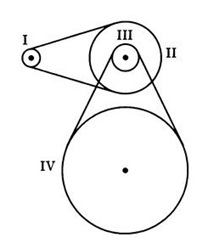
\includegraphics[width=0.8\linewidth]{chapters/chapter6/images/5}
			\caption{К задаче \Roman{tasks}.}
			\label{ris:image6x5}
		\end{center}
	\end{figure}
	\item Циркулярная пила имеет диаметр 600 мм. На ось пилы насажен шкив диаметром 300 мм, который приводится во вращение посредством ременной передачи от шкива диаметром 120 мм, насаженного на вал электродвигателя. Какова скорость зубьев пилы, если вал двигателя совершает 1200 об/мин?
	\item Диаметр колеса велосипеда «Пенза» d = 70 см, ведущая зубчатка имеет г1 = 48 зубцов, а ведомая z2 = 18 зубцов. С какой скоростью движется велосипедист на этом велосипеде при частоте вращения педалей п = 1 об/с? С какой скоростью движется велосипедист на складном велосипеде «Кама» при той же частоте вращения педалей, если у этого велосипеда соответственно d = 50 см, г1 = 48 зубцов, z2 = 15 зубцов?
\end{itemize}
\clearpage
{\hypertarget{lesson6x5}{\blackBlueText{V. Запускающий механизм волчка}}}\\\\

Для лучшего понимания понятий передаточное соотношение, повышающая передача предлагается провести следующее соревнование.

Каждому учащемуся предлагается собрать волчок из оси, насадив на нее колесо, как показано на рисунке.
\begin{figure}[h!]
	\begin{center}
		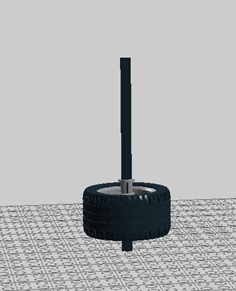
\includegraphics[width=0.8\linewidth]{chapters/chapter6/images/6}
		\caption{}
		\label{ris:image6x6}
	\end{center}
\end{figure}

Такой волчок можно легко запустить  рукой и он будет вращаться  10--20 секунд. Что нужно сделать, чтобы увеличить время вращения волчка? Ответ очевиден~--- изначально раскрутить его посильнее. Для этого мы сконструируем специальный механизм запускающий волчок.
\clearpage
\begin{figure}[h!]
	\begin{center}
		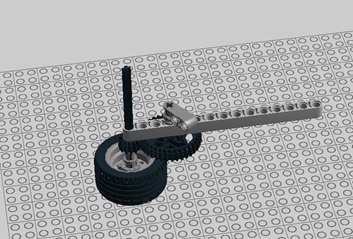
\includegraphics[width=0.9\linewidth]{chapters/chapter6/images/7}
		\caption{}
		\label{ris:image6x7}
	\end{center}
\end{figure}
\begin{figure}[h!]
	\begin{center}
		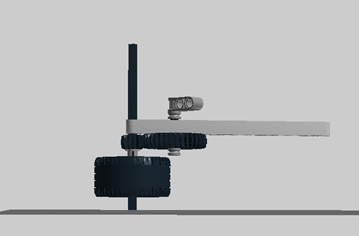
\includegraphics[width=0.9\linewidth]{chapters/chapter6/images/8}
		\caption{}
		\label{ris:image6x8}
	\end{center}
\end{figure}

Теперь пальцы раскручивают большую шестеренку, которая передает вращение маленькой, на оси волчка. У нас получилась повышающая передача с коэффициентом \greenText{столько-то}.

Теперь можно предложить детям собрать запускающие устройства с большим количеством шестеренок и устроить соревнования! Побеждает тот, чей волчок вращается дольше всего.

{\slshape Из набора 8547 можно собрать запускающее устройство с передаточным соотношением \greenText{столько-то}. Однако, для прокручивания первой шестеренки в таком случае нам надо приложить в \greenText{столько-то} же раз большую силу, а ведь есть еще и неучтенные нами потери на трение деталей друг о друга. Поэтому самый оптимальный с практической точки зрения механизм оказывается двухступенчатым:	
	\begin{figure}[h!]
		\begin{center}
			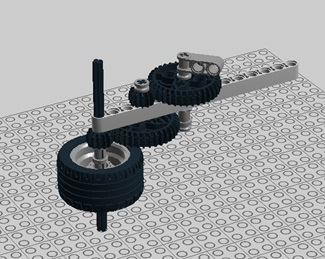
\includegraphics[width=1\linewidth]{chapters/chapter6/images/9}
			\caption{}
			\label{ris:image6x9}
		\end{center}
	\end{figure}
	
	Время вращения при этом доходит до \greenText{столько-то} секунд.}